\chapter{低温下的电子序}\label{chap:low-and-super}

很多集体行为和相变均可以通过经典的金斯堡-朗道理论加以描述:相变的出现是因为某个对称性(由于一些特殊的相互作用)被破缺了,然后我们可以使用某个序参量来描述相变,而序参量的涨落就给出了相变之后产生的元激发。
我们可以使用Hubbard-Stratonovich变换将二体相互作用解耦,适当选取Hubbard-Stratonovich参量使之和序参量对应,然后积掉电子自由度和声子自由度,这样就得到了元激发的有效理论。
序参量应该是通常是一些电子场算符的乘积或其线性组合,元激发是序参量的涨落,即元激发实际上是多个电子(或者也许还有声子或其他粒子)的集体行为,或者说\concept{粒子凝聚}。
此时的系统不再是一个普通的费米液体了,我们也可以说,\emph{特殊的相互作用通道让费米液体不稳定}。

费米子体系中可以有各种各样的这种电子凝聚:自旋密度波%
\footnote{
    为了避免引起混淆我们要区分自旋密度波和自旋波。后者是一个自旋系统中的现象,前者是一个费米子系统中的现象。
    或者,更加形象地说,后者是固定在格点上的自旋的空间涨落,前者是可以运动的、携带自旋的费米子密度的空间涨落。
}%
、电荷密度波、超导配对等。电子配对顾名思义,可能导致可以不受阻碍地随意移动的“超导电子”出现;所谓密度波实际上就是一种长程序,它在空间中有一种周期性振荡,可以是相位的振荡也可以是大小的振荡,
也即,这样的长程序对应的序参量形如%
\footnote{请注意这个序参量实际上是一种二电子集体运动模式,即相邻的两个电子的自旋总是保持一上一下的这种运动模式。
这暗示我们,如果需要超越平均场近似的理论,只需要把这种模式定义成一个新的(玻色)场就可以。
这个技巧和一维电子系统的玻色化很相似。}%
\begin{equation}
    \Delta(\vb*{r}) \sim \Delta_0 \ee^{\ii \vb*{Q} \cdot \vb*{r}}.
\end{equation}
这些现象对应的序参量对应于Hubbard-Stratonovich参量的不同选择;换句话说,不同的相互作用通道相互竞争,最终哪一种相互作用通道占据优势——从而,单单考虑它得到的相变出现——取决于很多条件。

应当指出的是这个图像并不能覆盖所有相变。例如在

\section{BCS超导}\label{sec:bcs-theory}

本节介绍一种常见的超导机制,即交换声子导致电子出现有效吸引相互作用而产生的BCS超导。

\subsection{交换声子导致的有效电子吸引相互作用}\label{sec:phonon-caused-interaction}

电子-声子相互作用的顶角为一个电子入射,一个电子出射,产生/消灭一个声子。
现在尝试积掉声子。我们先将电子场当成给定的,则可以从\eqref{eq:simple-phonon-electron-int}写出声子场加上电子-声子相互作用的虚时间作用量。本节仅考虑晶格是简单正方晶格的情况,于是没有各向异性,我们有
\[
    S_\text{ph} + S_\text{int} = \sum_{\omega_n, \vb*{q}, \lambda} \Big(
        \bar{\phi}_{\vb*{q} \lambda} (- \ii \omega_n + \omega_q) \phi_{\vb*{q} \lambda}
        + \gamma \frac{\ii q_\lambda}{\sqrt{2 M \omega_q}} (\phi_{\vb*{q} \lambda} + \bar{\phi}_{-\vb*{q} \lambda}) \underbrace{\sum_{\vb*{k}, \sigma} \bar{\psi}_{(\vb*{k} + \vb*{q}) \sigma} \psi_{\vb*{k} \sigma}}_{\rho_{\vb*{q}}}
    \Big),
\]
其中$\phi$表示声子,$\psi$表示电子。使用处理自由场受到线性激励的方法,配平方并积掉二次方项,忽略产生的因子,得到
\begin{equation}
    \begin{aligned}
        S_\text{eff} &= - \sum_{\omega_n, \vb*{q}} \frac{\gamma^2 q^2 \rho_{\vb*{q}} \rho_{-\vb*{q}}}{2 M \omega_q (\omega_q - \ii \omega_n)} 
        = - \sum_{\omega_n, \vb*{q}} \frac{\gamma^2 q^2 \rho_{\vb*{q}} \rho_{-\vb*{q}}}{2 M (\omega_q^2 + \omega_n^2)} \\ 
        &= - \frac{\gamma^2}{2 M} \sum_{\omega_n} \sum_{\vb*{q}, \vb*{k}, \vb*{k}', \alpha, \beta} \frac{q^2}{\omega_n^2 + \omega_q^2} \bar{\psi}_{(\vb*{k}+\vb*{q}) \alpha} \bar{\psi}_{(\vb*{k}' - \vb*{q}) \beta} \psi_{\vb*{k}' \beta} \psi_{\vb*{k} \alpha} .
    \end{aligned}
    \label{eq:retarded-two-electron}
\end{equation}
第二个等号是考虑到每个$\omega_n$有一个对应的$-\omega_n$而得到的。总之,电子之间可以通过交换声子来产生一个四电子相互作用。
相互作用\eqref{eq:retarded-two-electron}是推迟相互作用,因此原则上不能够仅仅使用一个哈密顿量描述。
不过,在推迟不明显时我们还是可以近似写出一个哈密顿量。这里有一个微妙的地方:\eqref{eq:retarded-two-electron}是定义在虚时间下的,即算符的时间演化为$\ee^{\omega t}$,而我们需要一个实时间下的哈密顿量,所以需要首先做频率上的Wick转动$\omega = \ii \omega_n$,得到
\[
    S_\text{eff}^\text{real} = - \frac{\gamma^2}{2 M} \int \dd{\omega} \sum_{\vb*{q}, \vb*{k}, \vb*{k}', \alpha, \beta} \frac{q^2}{- \omega^2 + \omega_q^2} \bar{\psi}_{(\vb*{k}+\vb*{q}) \alpha} \bar{\psi}_{(\vb*{k}' - \vb*{q}) \beta} \psi_{\vb*{k}' \beta} \psi_{\vb*{k} \alpha}.
\]
上式中的所有$\psi$都是$\omega$的函数,可以将它们转换到时域;我们也知道,上式的无推迟近似是它的无时间变化的傅里叶分量。
因此实际上我们只需要简单地取
\begin{equation}
    \omega = \epsilon_{\vb*{k}} - \epsilon_{\vb*{k} + \vb*{q}},
    \label{eq:phonon-introduced-omega}
\end{equation}
就得到了无推迟的近似
\begin{equation}
    \begin{aligned}
        {H} &= - \frac{\gamma^2}{2 M} \sum_{\vb*{q}, \vb*{k}, \vb*{k}', \alpha, \beta} \frac{q^2}{- \omega^2 + \omega_q^2} {c}^\dagger_{(\vb*{k}+\vb*{q}) \alpha} {c}^\dagger_{(\vb*{k}' - \vb*{q}) \beta} {c}_{\vb*{k}' \beta} {c}_{\vb*{k} \alpha} \\
        &= \frac{\gamma^2}{2 M} \sum_{\vb*{q}, \vb*{k}, \vb*{k}', \alpha, \beta} \frac{q^2}{(\epsilon_{\vb*{k}} - \epsilon_{\vb*{k}+\vb*{q}})^2 - \omega_q^2} {c}^\dagger_{(\vb*{k}+\vb*{q}) \alpha} {c}^\dagger_{(\vb*{k}' - \vb*{q}) \beta} {c}_{\vb*{k}' \beta} {c}_{\vb*{k} \alpha}.
    \end{aligned}
\end{equation}

更加一般地,设声子频率为$\omega_{\vb*{q}}$,电子-声子相互作用为
\begin{equation}
    H = \frac{1}{\sqrt{N}} \sum_{\vb*{k}, \vb*{q}} M_{\vb*{q}} c^\dagger_{\vb*{k} + \vb*{q}} c_{\vb*{k}} (b_{\vb*{q}} + b_{-\vb*{q}}^\dagger),
\end{equation}
重复以上步骤将得到% TODO
\begin{equation}
    {H}_{4\text{e}} = \frac{1}{2N} \sum_{\vb*{k}, \vb*{k}', \vb*{q}'} \sum_{\alpha, \beta} \abs{M_{\vb*{q}}}^2 \frac{\omega_{\vb*{q}}}{(\epsilon_{\vb*{k}} - \epsilon_{\vb*{k}+\vb*{q}})^2 - \omega_{\vb*{q}}^2} {c}^\dagger_{(\vb*{k}+\vb*{q}) \alpha} {c}^\dagger_{(\vb*{k}'-\vb*{q}) \beta} {c}_{\vb*{k}' \beta} {c}_{\vb*{k} \alpha},
    \label{eq:4-electron-interaction-by-phonon}
\end{equation}
其中$\omega_{\vb*{q}}$表示声子能量。任何更复杂的含有声子的费曼图都可以化归为二电子和声子的相互作用和一些电子相互作用的组合,因此\eqref{eq:4-electron-interaction-by-phonon}就给出了完整的没有声子的有效理论。
\eqref{eq:4-electron-interaction-by-phonon}本身是瞬时的,但即使我们不知道它来自一个推迟相互作用,\eqref{eq:4-electron-interaction-by-phonon}含有电子能量差而\eqref{eq:phonon-introduced-omega}也有这一事实也暗示它有可能实际上代表一个推迟相互作用。
另一方面,库伦势则没有推迟(当然这实际上做了近似,我们只不过不考虑相对论效应而已,但是电磁相互作用的推迟远小于声子传递导致的推迟)。

现在考虑一个低能有效理论%
\footnote{这就是超导往往发生在低温下的原因:否则没法形成电子的有效吸引,四散排斥的电子会造成很大耗散。}%
,其中我们需要考虑的过程全部发生在费米面附近,入射电子和出射电子能量都接近于$\epsilon_\text{F}$。
费米面是球形的,通过几何关系可以看出$\vb*{k} + \vb*{k}' = 0$的过程是最重要的,此时发生相互作用前两个电子始终在费米面的两端,相互作用之后两个电子还是位于费米面的两端。
这样\eqref{eq:4-electron-interaction-by-phonon}就简化为
\begin{equation}
    {H}_{4\text{e}} = \frac{1}{2N} \sum_{\vb*{k}, \vb*{q}'} \underbrace{\sum_{\alpha, \beta} \abs{M_{\vb*{q}}}^2 \frac{\omega_{\vb*{q}}}{(\epsilon_{\vb*{k}} - \epsilon_{\vb*{k}+\vb*{q}})^2 - \omega_{\vb*{q}}^2}}_{V(\vb*{q}, \epsilon_{\vb*{k}} - \epsilon_{\vb*{k}+\vb*{q}})} {c}^\dagger_{(\vb*{k}+\vb*{q}) \alpha} {c}^\dagger_{(-\vb*{k}-\vb*{q}) \beta} {c}_{-\vb*{k} \beta} {c}_{\vb*{k} \alpha}.
    \label{eq:low-energy-4-electron}
\end{equation}
由于电子能量差非常小,显然
\[
    V(\vb*{q}, \epsilon_{\vb*{k}} - \epsilon_{\vb*{k}+\vb*{q}}) = \abs{M_{\vb*{q}}}^2 \frac{\omega_{\vb*{q}}}{(\epsilon_{\vb*{k}} - \epsilon_{\vb*{k}+\vb*{q}})^2 - \omega_{\vb*{q}}^2} < 0,
\]
因此这个声子中介的相互作用是吸引相互作用。

库伦相互作用是排斥的,电-声子相互作用是吸引的;绝对强度显然是前者强。
然而,实际上库伦相互作用很容易被屏蔽,因为把低能电子看成外加电荷,那么高能电子就会来屏蔽它(见\autoref{sec:ext-e}),因此把高能电子积掉之后得到的屏蔽库仑相互作用并不强,因此在重整化下,库仑相互作用实际上只是对电子能带的修正(这和费米液体的想法很相似:渐染地加入一个不大的相互作用仅仅会导致电子自能修正而已)。
另一方面,电-声子相互作用是不容易屏蔽的,实际上推迟相互作用就是不容易屏蔽的。
因此,\eqref{eq:low-energy-4-electron}在重整化之后是主要的电子间相互作用。
还有一种看待这个问题的方式是,电-声子相互作用会导致有效的吸引,在重整化下一个吸引相互作用通常会导致粒子配对取代单粒子自由度成为主要的自由度,因此吸引相互作用不可能只是对能带的修正;库仑相互作用在这里是排斥的,不会造成粒子配对,因此正如Hartree-Fock近似中的那样,仅仅对电子能级产生了一个修正。

声子的频率只出现在0和德拜频率$\omega_\text{D}$之间,换而言之吸引相互作用只出现在
\[
    \omega = \abs{\epsilon_{\vb*{k}} - \epsilon_{\vb*{k}+\vb*{q}}} < \omega_\text{D}
\]
时。数值计算可以表明对超导现象而言最重要的是建立起电子之间的吸引相互作用,其具体形式并不重要,这是因为会参与超导的实际上只有费米面附近的非常小的一个能量范围内的电子,因此$V$的具体形式根本不重要,实际发挥作用的只有费米面上的$V$值。
这样我们设
\begin{equation}
    V(\vb*{q}, \omega) = \begin{cases}
        - V_0, \quad \omega < \omega_\text{D}, \\
        0, \quad \omega > \omega_\text{D}
    \end{cases}.
    \label{eq:superconductive-interaction-simplified}
\end{equation}
其中$\omega_\text{D}$是一个硬截断。这是一个非常粗糙的截断,但后面会发现它是合理的。
这样整个系统的哈密顿量就是
\begin{equation}
    {H} = \sum_{\vb*{k}, \alpha} (\epsilon_{\vb*{k}} - \mu) {c}_{\vb*{k} \alpha}^\dagger {c}_{\vb*{k} \alpha} - \frac{V_0}{2} \sum_{\vb*{k}, \vb*{q}} \sum_{\alpha, \beta} {c}^\dagger_{(\vb*{k} + \vb*{q}) \alpha} {c}^\dagger_{( - \vb*{k} - \vb*{q}) \beta} {c}_{-\vb*{k} \beta} {c}_{\vb*{k} \alpha}.
    \label{eq:simple-super-conductive-hamiltonian}
\end{equation}
$\vb*{k}$和$\vb*{k}+\vb*{q}$都在费米面附近。

\subsection{库伯对}

数值计算或者手算二体问题会发现可能出现\concept{库伯对},即一对位于费米面上的电子配对。
这种配对写成算符形式就是${c}^\dagger {c}^\dagger$的形式,或者等价的${c} {c}$形式。
如果其期望值不为零,那么$U(1)$对称性就破缺了,即电荷守恒对称性被破缺了(物理图像是,一部分电荷被封存到了库伯对中,不再以独立电子的形式流动)。我们会看到电荷守恒的破缺实际上是低温超导中最重要的物理。
于是,库伯对序参量的一般形式显然是$\expval*{{c}_{\vb*{k}\alpha} {c}_{\vb*{k}' \beta}}$。

现在我们做对称性分析。注意到时间反演对称性要求
\[
    \epsilon_{\vb*{k} \uparrow} = \epsilon_{-\vb*{k} \downarrow},
\]
而\eqref{eq:simple-super-conductive-hamiltonian}中单电子能量和自旋无关,于是
\[
    \epsilon_{\vb*{k}} = \epsilon_{-\vb*{k}}.
\]
这样就容易验证\eqref{eq:simple-super-conductive-hamiltonian}在变换$\vb*{k} \longrightarrow -\vb*{k}$下不变,这个对称性没有被破缺掉,于是
\[
    \expval*{{c}_{\vb*{k}\alpha} {c}_{\vb*{k}' \beta}} \propto \delta(\vb*{k} + \vb*{k}').
\]
换而言之,我们只考虑总动量为零的配对$\expval*{{c}_{\vb*{k} \alpha} {c}_{- \vb*{k} \beta}}$。
此外还可以发现\eqref{eq:simple-super-conductive-hamiltonian}具有自旋旋转不变性,因此相应的序参量$\expval*{{c}_{\vb*{k} \alpha} {c}_{- \vb*{k} \beta}}$应该是一个二分量的自旋协变的对象。二粒子配对对应的$SU(2)$的表示为
\[
    \frac{1}{2} \otimes \frac{1}{2} = 0 \oplus 1,
\]
即可能有自旋单态也可能有自旋三重态。如果该库伯对是自旋单态,那么应该有
\[
    \expval*{{c}_{\vb*{k} \alpha} {c}_{- \vb*{k} \beta}} \propto \epsilon_{\alpha \beta} \propto \delta_{\alpha+\beta,0},
\]
其中$\epsilon$为所谓的旋量度规;而如果该库珀对为自旋三重态,那么就应该有
\[
    \expval*{{c}_{\vb*{k} \alpha} {c}_{- \vb*{k} \beta}} \propto \vb*{d} \cdot \vb*{\sigma}_{\alpha \beta}.
\]
% TODO:为什么??
最后,由于没有自旋-轨道耦合,$\expval*{{c}_{\vb*{k} \alpha} {c}_{- \vb*{k} \beta}}$可以写成“动量部分乘以自旋部分”的形式。
这样我们设
\[
    \expval*{{c}_{\vb*{k} \alpha} {c}_{- \vb*{k} \beta}} \propto \Delta(\vb*{k}).
\]
如果该库伯对是自旋单态的,那么其自旋部分是反对称的,则其轨道部分就是对称的,也即
\[
    \Delta(\vb*{k}) = \Delta(-\vb*{k}),
\]
从而可以将$\Delta(\vb*{k})$展开成一系列s波、d波等对称球谐函数的线性组合;
而如果该库伯对是自旋三重态的,那么其自旋部分就是对称的,于是轨道部分满足
\[
    \Delta(\vb*{k}) = -\Delta(-\vb*{k}),
\]
此时$\Delta(\vb*{k})$是一系列反对称球谐函数的线性组合。
容易看出单态或者三重态的出现和费米面对称性的关系,比如如果费米面不对称,那么s波配对就不能产生。

\subsection{平均场近似和Bogoliubov变换}

对\eqref{eq:simple-super-conductive-hamiltonian}做平均场近似,有
\[
    \begin{aligned}
        & \quad {c}^\dagger_{(\vb*{k} + \vb*{q}) \alpha} {c}^\dagger_{( - \vb*{k} - \vb*{q}) \beta} {c}_{-\vb*{k} \beta} {c}_{\vb*{k} \alpha} \\
        &\approx \expval*{{c}^\dagger_{(\vb*{k} + \vb*{q}) \alpha} {c}^\dagger_{( - \vb*{k} - \vb*{q}) \beta}} {c}_{-\vb*{k} \beta} {c}_{\vb*{k} \alpha} + {c}^\dagger_{(\vb*{k} + \vb*{q}) \alpha} {c}^\dagger_{( - \vb*{k} - \vb*{q}) \beta} \expval*{{c}_{-\vb*{k} \beta} {c}_{\vb*{k} \alpha}} - \expval*{{c}^\dagger_{(\vb*{k} + \vb*{q}) \alpha} {c}^\dagger_{( - \vb*{k} - \vb*{q}) \beta} {c}_{-\vb*{k} \beta} {c}_{\vb*{k} \alpha}},
    \end{aligned}
\]
重新选定求和哑指标,并略去对体系动力学没有影响的常数项,得到
\begin{equation}
    {H}_\text{MF} = \sum_{\vb*{k}, \alpha} (\epsilon_{\vb*{k}} - \mu) {c}_{\vb*{k} \alpha}^\dagger {c}_{\vb*{k} \alpha} - \frac{V_0}{2} \sum_{\vb*{k}, \vb*{k}', \alpha, \beta} \left(
        \expval*{{c}_{-\vb*{k} \beta} {c}_{\vb*{k} \alpha}} {c}^\dagger_{\vb*{k}' \alpha} {c}^\dagger_{- \vb*{k}' \beta} + \text{h.c.} 
    \right).
\end{equation}
的确,电荷守恒对称性被破缺了,原因是电子形成库伯对之后看起来就像被“冻结”了一样,因此不再被计入${c}^\dagger$自由度中,而是被计入序参量$\expval*{{c}_{-\vb*{k} \beta} {c}_{\vb*{k} \alpha}}$中。

现在我们考虑单态、s波的库伯对,这样发生配对的就是一个$\vb*{k}, \uparrow$态的电子和一个$-\vb*{k}, \downarrow$态的电子,或者做一个自旋旋转。总之,序参量可以选取为
\begin{equation}
    \Delta = - \frac{V_0}{2} \sum_{\vb*{k}} (
        \expval*{{c}_{-\vb*{k}\uparrow} {c}_{\vb*{k} \downarrow}} - \expval*{{c}_{-\vb*{k} \downarrow} {c}_{\vb*{k} \uparrow}}
    ) = -V_0 \sum_{\vb*{k}} \expval*{{c}_{-\vb*{k}\uparrow} {c}_{\vb*{k} \downarrow}} ,
    \label{eq:superconductive-order-parameter}
\end{equation}
则可以证明
\begin{equation}
    {H}_\text{MF} = \sum_{\vb*{k}, \alpha} \xi_{\vb*{k}} {c}_{\vb*{k} \alpha}^\dagger {c}_{\vb*{k} \alpha} 
    + \Delta \sum_{\vb*{k}} {c}_{-\vb*{k} \downarrow}^\dagger {c}^\dagger_{\vb*{k} \uparrow}
    + \Delta^* \sum_{\vb*{k}} {c}_{\vb*{k} \uparrow} {c}_{-\vb*{k} \downarrow}.
    \label{eq:s-wave-superconductive-hamiltonian}
\end{equation}

在\eqref{eq:s-wave-superconductive-hamiltonian}中总是可以对${c}$和${c}^\dagger$做一个幺正变换,让$\Delta$为实数,因此以下假定$\Delta$为实数。
用一个幺正变换重新定义一组准粒子(这就称为\concept{Bogoliubov变换}),使这组准粒子本身是费米子,并且能够让\eqref{eq:s-wave-superconductive-hamiltonian}对角化(从而这组准粒子的能谱就是\eqref{eq:s-wave-energy-band})。
首先我们有费米子的对易关系
\[
    \acomm*{{\gamma}_{\vb*{k}_1 \alpha}}{{\gamma}^\dagger_{\vb*{k}_2 \beta}} = \delta_{\vb*{k}_1 \vb*{k}_2} \delta_{\alpha \beta}, \quad \acomm*{{\gamma}_{\vb*{k}_1 \alpha}}{{\gamma}_{\vb*{k}_2 \beta}} = 0,
\]
并且可以看到,以下正交变换
\[
    \pmqty{{\gamma}_{\vb*{k} \uparrow} \\ {\gamma}^\dagger_{-\vb*{k} \downarrow}} = \pmqty{u_{\vb*{k}} & -v_{\vb*{k}} \\ v_{\vb*{k}} & u_{\vb*{k}}} \pmqty{{c}_{\vb*{k} \uparrow} \\ {c}^\dagger_{-\vb*{k} \downarrow}},
    \quad u_{\vb*{k}}^2 + v_{\vb*{k}}^2 = 1
\]
能够给出正确的对易关系,则可以解出
\begin{equation}
    u_{\vb*{k}} = \sqrt{\frac{E_{\vb*{k}} + \xi_{\vb*{k}}}{2 E_{\vb*{k}}}}, \quad v_{\vb*{k}} = \sqrt{\frac{E_{\vb*{k}} - \xi_{\vb*{k}}}{2 E_{\vb*{k}}}}.
\end{equation}
这就得到了Bogoliubov变换的显式形式:
\begin{equation}
    \begin{cases}
        {\gamma}_{\vb*{k} \uparrow} = u_{\vb*{k}} {c}_{\vb*{k} \uparrow} - v_{\vb*{k}} {c}_{-\vb*{k} \downarrow}^\dagger, \\
        {\gamma}_{\vb*{k} \downarrow} = u_{\vb*{k}} {c}_{\vb*{k} \downarrow} + v_{\vb*{k}} {c}_{-\vb*{k} \uparrow}^\dagger,
    \end{cases}
    \label{eq:bogoliubov-transform}
\end{equation}
还有它的逆变换
\begin{equation}
    \begin{cases}
        {c}_{\vb*{k} \uparrow} = u_{\vb*{k}} {\gamma}_{\vb*{k} \uparrow} + v_{\vb*{k}} {\gamma}_{-\vb*{k} \downarrow}^\dagger, \\
        {c}_{\vb*{k} \downarrow} = u_{\vb*{k}} {\gamma}_{\vb*{k} \downarrow} - v_{\vb*{k}} {\gamma}_{-\vb*{k} \uparrow}^\dagger.
    \end{cases}
    \label{eq:inverse-bogoliubov-transform}
\end{equation}
由于从${c}$到${\gamma}$的线性变换是一个正交变换%
\footnote{这件事不是一般成立的,有时候真的要用一个非正交变换;关键在于对易关系必须正确,不是所有的线性变换形式都能够给出正确的对易关系。}%
,\eqref{eq:s-wave-superconductive-hamiltonian}的能谱可以通过对角化矩阵的方式求出。
求解之后会发现能带为
\begin{equation}
    E_{\vb*{k}} = \pm \sqrt{ \xi_{\vb*{k}}^2 + \abs{\Delta}^2 }.
    \label{eq:s-wave-energy-band}
\end{equation}
这个结果具有粒子-空穴对称性,但是这并不具有太多物理意义,因为它实际上是对角化时交换了一对产生湮灭算符,从而把一部分粒子自由度写成了空穴而已。
\eqref{eq:s-wave-energy-band}中,序参量$\Delta$把原本发生交叉的两条能带$E=\pm \xi_{\vb*{k}}$的交叉点分开了,即打开了一个能隙。

% TODO:系统基态

\subsection{平均场自洽计算}

得到平均场理论后我们来做自洽计算。将\eqref{eq:inverse-bogoliubov-transform}代入\eqref{eq:superconductive-order-parameter},并利用近独立电子气的数目
\[
    \expval*{{\gamma}_{\vb*{k} \alpha}^\dagger {\gamma}_{\vb*{k} \alpha}} = n_\text{F}(E_{\vb*{k}}) =  \frac{1}{\ee^{\beta E_{\vb*{k}}} + 1},
\]
得到
\[
    \Delta = - V_0 \sum_{\vb*{k}} u_{\vb*{k}} v_{\vb*{k}} (2 n_\text{F}(E_{\vb*{k}}) - 1).
\]
可以验证,
\[
    u_{\vb*{k}} v_{\vb*{k}} = \frac{\Delta}{2 E_{\vb*{k}}},
\]
于是最终得到
\begin{equation}
    \Delta V_0 \sum_{\vb*{k}} \frac{1}{2 E_{\vb*{k}}} \frac{\ee^{\beta E_{\vb*{k}}} - 1}{\ee^{\beta E_{\vb*{k}}} + 1} = \Delta.
    \label{eq:superconductive-self-consistency}
\end{equation}
如果$\Delta$为零,即出现超导现象,就可以把$\Delta$消掉。$E_{\vb*{k}}$依赖于$\Delta$,于是给定一个温度就可以把$\Delta$解出。

例如,在$T=0$时,我们有
\[
    1 = V_0 \sum_{\vb*{k}} \frac{1}{2 E_{\vb*{k}}} = V_0 \int \dd{\epsilon} N(\epsilon) \frac{1}{2 \sqrt{\epsilon^2 + \Delta^2}},
\]
这里我们在对单个电子的能量做积分。当然由于电子能量过高时\autoref{sec:phonon-caused-interaction}中的机制不再适用,积分能量肯定有一个截断。
\eqref{eq:superconductive-interaction-simplified}给出了截断$\omega_\text{D}$。我们假定$\omega_\text{D}$相对费米能非常小,也即发生库伯配对的电子只是费米面附近非常小的一个能量范围内的,则近似有
\[
    1 = V_0 N(0) \int_{-\omega_\text{D}}^{\omega_\text{D}} \dd{\epsilon} \frac{1}{\sqrt{\epsilon^2 + \Delta^2}} = N(0) V_0 \sinh^{-1} \left( \frac{\omega_\text{D}}{\Delta} \right) \approx N(0) V_0 \ln \frac{2 \omega_\text{D}}{\Delta},
\]
于是
\begin{equation}
    \Delta = 2 \omega_\text{D} \exp(- \frac{1}{N(0) V_0}).
\end{equation}
显然,$\Delta$对$V_0$的依赖比对$\omega_\text{D}$的依赖要强得多。这是合理的,因为$\omega_\text{D}$实际上是一个非常粗糙的硬截断。
现在我们看到,硬截断\eqref{eq:superconductive-interaction-simplified}是合理的,因为截断只是给$\Delta$提供了一个能量尺度而已,不会影响更为复杂的行为。
我们也可以看出,只要有相互作用,不管多强,都会产生一个非零的$\Delta$,因此只要有相互作用就会出现超导转变,并打开能隙。
这意味着\eqref{eq:4-electron-interaction-by-phonon}具有非微扰行为。

\eqref{eq:superconductive-self-consistency}中总是有一个平庸解$\Delta = 0$,消掉因子$\Delta$之后得到的方程就不总是有解。
消掉因子$\Delta$之后得到的方程有没有解就区分了超导相和非超导相。
现在我们计算临界温度,即$\Delta$从非零的一侧趋于零时的温度:
\[
    \begin{aligned}
        1 &= \lim_{\Delta \to 0} V_0 \sum_{\vb*{k}} \frac{1}{2 E_{\vb*{k}}} \frac{\ee^{\beta E_{\vb*{k}}} - 1}{\ee^{\beta E_{\vb*{k}}} + 1} \\
        &= V_0 \sum_{\vb*{k}} \frac{1}{2 \xi_{\vb*{k}}} \frac{\ee^{\beta \xi_{\vb*{k}}} - 1}{\ee^{\beta \xi_{\vb*{k}}} + 1} \\
        &= V_0 \int_{-\omega_\text{D}}^{\omega_\text{D}} \dd{\epsilon} N(\epsilon) \frac{1}{2 \epsilon} \frac{\ee^{\beta \epsilon} - 1}{\ee^{\beta \epsilon} + 1} \\
        &\approx V_0 N(0) \int_{0}^{\omega_\text{D}} \dd{\epsilon} \frac{1}{\epsilon} \frac{\ee^{\beta \epsilon} - 1}{\ee^{\beta \epsilon} + 1}.
    \end{aligned}
\]
最后一个积分中的因子$(\ee^{\beta \epsilon} - 1) / (\ee^{\beta \epsilon} + 1)$的作用在于在$\epsilon$接近$0$时压低$1/\epsilon$的值从而避免发散,它是一个特征尺度为$\beta$的红外截断,于是
\[
    1 \sim V_0 N(0) \int_{\beta}^{\omega_\text{D}} \dd{\epsilon} \frac{1}{\epsilon},
\]
最后得到
\begin{equation}
    T_\text{c} \sim \frac{\omega_\text{D}}{k_\text{B}} \exp \left( - \frac{1}{N(0) V_0} \right).
\end{equation}
更为精确的计算会给出
\begin{equation}
    T_\text{c} = 1.14 \frac{\omega_\text{D}}{k_\text{B}} \exp \left( - \frac{1}{N(0) V_0} \right),
\end{equation}
不过实际上以上公式自身不大,因为首先很难精确计算$V_0$,其次$V_0$的微小变化会带来很大误差。
真正会在实验上验证的通常是
\begin{equation}
    \frac{2 \Delta(T=0)}{k_\text{B} T_\text{c}} = 3.5.
\end{equation}
如果实验测量出来的比值远离3.5,那就可以确定这个超导现象不来自BCS机制。

\subsection{朗道-金斯堡理论}

现在我们采取另一条路,尝试直接从$U(1)$对称性被破缺这件事来获得关于超导的一些解释。
设$\Phi$为库伯对序参量,我们知道它是一个复标量场。有时称它为超导波函数,虽然它并不是任何粒子的波函数,但它服从的方程和薛定谔方程形式一致。
我们假定超导相中仅有的重要的自由度是这个序参量,其他量(比如单个电子)全部不重要。%
\footnote{这个假设是整个理论中最需要物理直觉的部分,因为并非对全部体系都有这个结论,例如做一维电子的玻色化时就不能只用一个标量场,在分析二维正方晶格的自旋波时也需要同时考虑序参量和电子。
在讨论BCS系统时能用这个假设是因为如前所述,破缺的是$U(1)$对称性,而$U(1)$对称性被破缺是因为电子在低温下配对为库伯对。
这个机制才是最关键的,因为它表明没有必要考虑单个电子的行为,电子的全部行为都被库伯对反映了,因此只需要考虑库伯对序参量即可。}%
设外加一个大小为$\vb*{A}$的磁矢势,按照规范不变性我们写下一个理论
\begin{equation}
    F = \int \dd[3]{\vb*{r}} \left( \abs*{(\grad - \ii 2 e \vb*{A}) \Phi}^2 + r \abs{\Phi}^2 + u\abs{\Phi}^4 \right).
    \label{eq:gl-theory}
\end{equation}
这里我们已经使用协变导数代替了原有的导数;系数为$2e$是因为一个库伯对带有两个负电荷,或者更加数学地说,一个库伯对包含两个湮灭算符,因此做$U(1)$变换时会有两个复数因子而不只是一个。
\eqref{eq:gl-theory}在相变点附近保证成立,一方面,相变点附近库伯对序参量不大,可以级数展开取前几项,另一方面,通过量纲分析可以发现
\[
    [\Phi] \sim [L]^{-1/2},
\]
容易验证没有提到的项在重整化不动点附近全部是不相关的,在重整化群作用下会被压低。
我们遵从做朗道-金斯堡理论时的惯例,适当调节单位制来让梯度平方项前面的系数为1。

计算\eqref{eq:gl-theory}的极小值点,可以得到
\begin{equation}
    - \frac{(\grad - \ii e \vb*{A})^2}{4 m^*} \Phi + \alpha \Phi + \beta \abs{\Phi}^2 \Phi = 0.
\end{equation}
这个方程的形式和薛定谔方程非常接近,当然这更多是对称性带来的结果,即薛定谔场也具有$U(1)$对称性。

$U(1)$对称性给出的守恒流为
\begin{equation}
    \vb*{j} \propto \Phi^* \grad{\Phi} - \Phi \grad{\Phi^*},
\end{equation}
当然这就是电流。当然,由于我们只是在做对称性分析,并不能明确地得出式子右边的系数。
上式说明超导的电流来自序参量的梯度,这和通常导电的机制(电场下费米面发生移动)不同。由于序参量是复的,即使不存在振幅输运,仅仅靠不同点相位不同就足够产生持续电流。这是一个稳态解,所以不存在能量消耗。这也就是超导体唯象地看起来似乎有某种运动全然不会受到阻碍的“反常电子”的原因。

\section{二维正方晶格的反铁磁长程序}

\subsection{二维正方晶格上的自旋}

\begin{figure}
    \centering
    \subfigure[自旋密度波]{
        

\tikzset{every picture/.style={line width=0.75pt}} %set default line width to 0.75pt        

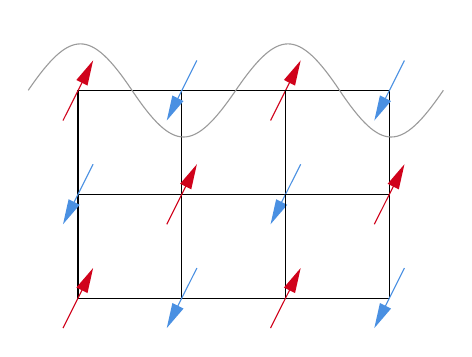
\begin{tikzpicture}[x=0.75pt,y=0.75pt,yscale=-1,xscale=1]
%uncomment if require: \path (0,300); %set diagram left start at 0, and has height of 300

%Shape: Square [id:dp7968380272014384] 
\draw   (148,62) -- (198,62) -- (198,112) -- (148,112) -- cycle ;
%Shape: Square [id:dp08936498453558128] 
\draw   (98,62) -- (148,62) -- (148,112) -- (98,112) -- cycle ;
%Shape: Square [id:dp6338164799723338] 
\draw   (98,112) -- (148,112) -- (148,162) -- (98,162) -- cycle ;
%Shape: Square [id:dp5647790600566112] 
\draw   (148,112) -- (198,112) -- (198,162) -- (148,162) -- cycle ;
%Straight Lines [id:da4505706138663077] 
\draw [color={rgb, 255:red, 208; green, 2; blue, 27 }  ,draw opacity=1 ]   (90.75,76.46) -- (104.35,49.33) ;
\draw [shift={(105.25,47.54)}, rotate = 476.63] [fill={rgb, 255:red, 208; green, 2; blue, 27 }  ,fill opacity=1 ][line width=0.08]  [draw opacity=0] (12,-3) -- (0,0) -- (12,3) -- cycle    ;
%Straight Lines [id:da8302639980131186] 
\draw [color={rgb, 255:red, 74; green, 144; blue, 226 }  ,draw opacity=1 ]   (155.25,47.54) -- (141.65,74.67) ;
\draw [shift={(140.75,76.46)}, rotate = 296.63] [fill={rgb, 255:red, 74; green, 144; blue, 226 }  ,fill opacity=1 ][line width=0.08]  [draw opacity=0] (12,-3) -- (0,0) -- (12,3) -- cycle    ;
%Straight Lines [id:da07392319534895608] 
\draw [color={rgb, 255:red, 208; green, 2; blue, 27 }  ,draw opacity=1 ]   (140.75,126.46) -- (154.35,99.33) ;
\draw [shift={(155.25,97.54)}, rotate = 476.63] [fill={rgb, 255:red, 208; green, 2; blue, 27 }  ,fill opacity=1 ][line width=0.08]  [draw opacity=0] (12,-3) -- (0,0) -- (12,3) -- cycle    ;
%Straight Lines [id:da29949826504712806] 
\draw [color={rgb, 255:red, 208; green, 2; blue, 27 }  ,draw opacity=1 ]   (90.75,176.46) -- (104.35,149.33) ;
\draw [shift={(105.25,147.54)}, rotate = 476.63] [fill={rgb, 255:red, 208; green, 2; blue, 27 }  ,fill opacity=1 ][line width=0.08]  [draw opacity=0] (12,-3) -- (0,0) -- (12,3) -- cycle    ;
%Straight Lines [id:da10136846066630589] 
\draw [color={rgb, 255:red, 208; green, 2; blue, 27 }  ,draw opacity=1 ]   (190.75,76.46) -- (204.35,49.33) ;
\draw [shift={(205.25,47.54)}, rotate = 476.63] [fill={rgb, 255:red, 208; green, 2; blue, 27 }  ,fill opacity=1 ][line width=0.08]  [draw opacity=0] (12,-3) -- (0,0) -- (12,3) -- cycle    ;
%Straight Lines [id:da18679469569417329] 
\draw [color={rgb, 255:red, 74; green, 144; blue, 226 }  ,draw opacity=1 ]   (105.25,97.54) -- (91.65,124.67) ;
\draw [shift={(90.75,126.46)}, rotate = 296.63] [fill={rgb, 255:red, 74; green, 144; blue, 226 }  ,fill opacity=1 ][line width=0.08]  [draw opacity=0] (12,-3) -- (0,0) -- (12,3) -- cycle    ;
%Straight Lines [id:da9509291375625459] 
\draw [color={rgb, 255:red, 74; green, 144; blue, 226 }  ,draw opacity=1 ]   (155.25,147.54) -- (141.65,174.67) ;
\draw [shift={(140.75,176.46)}, rotate = 296.63] [fill={rgb, 255:red, 74; green, 144; blue, 226 }  ,fill opacity=1 ][line width=0.08]  [draw opacity=0] (12,-3) -- (0,0) -- (12,3) -- cycle    ;
%Shape: Square [id:dp7989800051587621] 
\draw   (198,62) -- (248,62) -- (248,112) -- (198,112) -- cycle ;
%Straight Lines [id:da025654938728039145] 
\draw [color={rgb, 255:red, 74; green, 144; blue, 226 }  ,draw opacity=1 ]   (205.25,97.54) -- (191.65,124.67) ;
\draw [shift={(190.75,126.46)}, rotate = 296.63] [fill={rgb, 255:red, 74; green, 144; blue, 226 }  ,fill opacity=1 ][line width=0.08]  [draw opacity=0] (12,-3) -- (0,0) -- (12,3) -- cycle    ;
%Shape: Square [id:dp21923612897643863] 
\draw   (198,112) -- (248,112) -- (248,162) -- (198,162) -- cycle ;
%Straight Lines [id:da2934635233522882] 
\draw [color={rgb, 255:red, 208; green, 2; blue, 27 }  ,draw opacity=1 ]   (190.75,176.46) -- (204.35,149.33) ;
\draw [shift={(205.25,147.54)}, rotate = 476.63] [fill={rgb, 255:red, 208; green, 2; blue, 27 }  ,fill opacity=1 ][line width=0.08]  [draw opacity=0] (12,-3) -- (0,0) -- (12,3) -- cycle    ;
%Straight Lines [id:da9412499087817388] 
\draw [color={rgb, 255:red, 74; green, 144; blue, 226 }  ,draw opacity=1 ]   (255.25,47.54) -- (241.65,74.67) ;
\draw [shift={(240.75,76.46)}, rotate = 296.63] [fill={rgb, 255:red, 74; green, 144; blue, 226 }  ,fill opacity=1 ][line width=0.08]  [draw opacity=0] (12,-3) -- (0,0) -- (12,3) -- cycle    ;
%Straight Lines [id:da18617934942542336] 
\draw [color={rgb, 255:red, 74; green, 144; blue, 226 }  ,draw opacity=1 ]   (255.25,147.54) -- (241.65,174.67) ;
\draw [shift={(240.75,176.46)}, rotate = 296.63] [fill={rgb, 255:red, 74; green, 144; blue, 226 }  ,fill opacity=1 ][line width=0.08]  [draw opacity=0] (12,-3) -- (0,0) -- (12,3) -- cycle    ;
%Straight Lines [id:da24257455825409324] 
\draw [color={rgb, 255:red, 208; green, 2; blue, 27 }  ,draw opacity=1 ]   (240.75,126.46) -- (254.35,99.33) ;
\draw [shift={(255.25,97.54)}, rotate = 476.63] [fill={rgb, 255:red, 208; green, 2; blue, 27 }  ,fill opacity=1 ][line width=0.08]  [draw opacity=0] (12,-3) -- (0,0) -- (12,3) -- cycle    ;
%Shape: Sine Wave Form [id:dp4769190459095818] 
\draw  [color={rgb, 255:red, 155; green, 155; blue, 155 }  ,draw opacity=1 ] (74,61.91) .. controls (94.35,32.16) and (103.94,32) .. (123.99,61.91) .. controls (144.06,91.82) and (153.47,92) .. (174,61.91) ;
%Shape: Sine Wave Form [id:dp8043046043167636] 
\draw  [color={rgb, 255:red, 155; green, 155; blue, 155 }  ,draw opacity=1 ] (174,61.91) .. controls (194.35,32.16) and (203.94,32) .. (223.99,61.91) .. controls (244.06,91.82) and (253.47,92) .. (274,61.91) ;




\end{tikzpicture}      
    }
    \subfigure[SDW形成后的两条子格子]{
        \documentclass[hyperref, UTF8, a4paper]{ctexart}

\usepackage{geometry}
\usepackage{titling}
\usepackage{titlesec}
\usepackage{paralist}
\usepackage{footnote}
\usepackage{enumerate}
\usepackage{amsmath, amssymb, amsthm}
\usepackage{bbm}
\usepackage{cite}
\usepackage{graphicx}
\usepackage{subfigure}
\usepackage{physics}
\usepackage{tikz}
\usepackage{autobreak}
\usepackage[ruled, vlined, linesnumbered, noend]{algorithm2e}
\usepackage[colorlinks, linkcolor=black, anchorcolor=black, citecolor=black]{hyperref}
\usepackage{prettyref}

% Page style
\geometry{left=3.18cm,right=3.18cm,top=2.54cm,bottom=2.54cm}
\titlespacing{\paragraph}{0pt}{1pt}{10pt}[20pt]
\setlength{\droptitle}{-5em}
\preauthor{\vspace{-10pt}\begin{center}}
\postauthor{\par\end{center}}

% Math operators
\DeclareMathOperator{\timeorder}{T}
\DeclareMathOperator{\diag}{diag}
\DeclareMathOperator{\legpoly}{P}
\DeclareMathOperator{\primevalue}{P}
\DeclareMathOperator{\sgn}{sgn}
\newcommand*{\ii}{\mathrm{i}}
\newcommand*{\ee}{\mathrm{e}}
\newcommand*{\const}{\mathrm{const}}
\newcommand*{\comment}{\paragraph{注记}}
\newcommand*{\suchthat}{\quad \text{s.t.} \quad}
\newcommand*{\argmin}{\arg\min}
\newcommand*{\argmax}{\arg\max}
\newcommand*{\normalorder}[1]{: #1 :}
\newcommand*{\pair}[1]{\langle #1 \rangle}
\newcommand*{\fd}[1]{\mathcal{D} #1}
\DeclareMathOperator{\bigO}{\mathcal{O}}

% prettyref setting
\newrefformat{sec}{第\ref{#1}节}
\newrefformat{note}{注\ref{#1}}
\newrefformat{fig}{图\ref{#1}}
\newrefformat{alg}{算法\ref{#1}}
\renewcommand{\autoref}{\prettyref}

% TikZ setting
\usetikzlibrary{arrows,shapes,positioning}
\usetikzlibrary{arrows.meta}
\usetikzlibrary{decorations.markings}
\tikzstyle arrowstyle=[scale=1]
\tikzstyle directed=[postaction={decorate,decoration={markings,
    mark=at position .5 with {\arrow[arrowstyle]{stealth}}}}]
\tikzstyle ray=[directed, thick]
\tikzstyle dot=[anchor=base,fill,circle,inner sep=1pt]

% Algorithm setting
\renewcommand{\algorithmcfname}{算法}
% Python-style code
\SetKwIF{If}{ElseIf}{Else}{if}{:}{elif:}{else:}{}
\SetKwFor{For}{for}{:}{}
\SetKwFor{While}{while}{:}{}
\SetKwInput{KwData}{输入}
\SetKwInput{KwResult}{输出}
\SetArgSty{textnormal}

\renewcommand{\emph}[1]{\textbf{#1}}
\newcommand*{\concept}[1]{\underline{\textbf{#1}}}
\newcommand*{\Ztwo}{$\mathbb{Z}_2$}

\title{常见格点模型}
\author{吴何友}

\begin{document}

\maketitle

\section{相互作用体系}

\subsection{Hubbard模型}

\concept{Hubbard模型}是一种常见的强关联电子模型,它是一个定义在点阵上的模型,以下我们照惯例用$i, j$等表示格点坐标。
不包含化学势的哈密顿量为
\begin{equation}
    \hat{H} = \underbrace{-t \sum_{\pair{i, j}, \sigma} \hat{c}_{i\sigma}^\dagger \hat{c}_{j\sigma} + \text{h.c.}}_{\hat{H}_0} + \underbrace{U \sum_i \hat{n}_{i \uparrow} \hat{n}_{i \downarrow}}_{\hat{H}_\text{I}}.
\end{equation}
或者,为了后面蒙特卡洛模拟的方便,重新定义化学势,也可以有
\begin{equation}
    \hat{H} = -t \sum_{\pair{i, j}, \sigma} \hat{c}_{i\sigma}^\dagger \hat{c}_{j\sigma} + \text{h.c.} 
    + U \sum_i \left(\hat{n}_{i\uparrow} - \frac{1}{2}\right) \left(\hat{n}_{i\downarrow} - \frac{1}{2}\right).
\end{equation}

\subsubsection{Hubbard模型的量子蒙特卡洛模拟}

\subsection{Trotter分解和辅助场引入}

下面我们尝试对Hubbard模型做Trotter分解。设虚时间间隔为$\Delta\tau$,总共有$m$个虚时间点,$\tau=m\Delta \tau$。
对Hubbard模型,有一种特殊的分解方法:
\begin{equation}
    \ee^{-\Delta \tau \hat{H}_\text{I}} = \gamma \sum_{s_1, s_2, \ldots, s_N = \pm 1} \ee^{\alpha \sum_i s_i (\hat{n}_{i\uparrow} - \hat{n}_{i \downarrow})}, 
    \quad \gamma = \frac{1}{2^N} \ee^{\Delta \tau U N / 4}, \quad \cosh(\alpha) = \ee^{\Delta \tau U / 2},
\end{equation}
可以看到$\gamma$是一个和辅助场$\{s_i\}$(照惯例我们下面记它的时间线为$\vb{s}$)无关的量,考虑到配分函数的常数因子无关紧要,略去此因子,则配分函数为
\[
    \begin{aligned}
        Z &= \trace \prod_{n=1}^m \sum_{\vb{s}_{n}} \ee^{\alpha \sum_i s_i (\hat{n}_{i\uparrow} - \hat{n}_{i \downarrow})} \ee^{\Delta \tau t \sum_{\pair{i, j}, \sigma} \hat{c}_{i\sigma}^\dagger \hat{c}_{j\sigma} + \text{h.c.}} \\
        &= \sum_{\vb{s}} \prod_{n=1}^m \ee^{\alpha \hat{c}^\dagger_{\uparrow} \diag{\vb{s}_n} \hat{c}_{\uparrow}} \ee^{- \alpha \hat{c}^\dagger_{\downarrow} \diag{\vb{s}_n} \hat{c}_{\downarrow}} \ee^{- \Delta \tau \hat{c}_\uparrow^\dagger \vb{T} \hat{c}_\uparrow} \ee^{- \Delta \tau \hat{c}_\downarrow^\dagger \vb{T} \hat{c}_\downarrow},
    \end{aligned}
\]
其中我们指定$\vb{T}$是动能部分$\hat{H}_0$在单粒子表象下的系数矩阵,即
\begin{equation}
    T_{ij} = \begin{cases}
        -t, \quad &\pair{i, j}, \\
        0, \quad &\text{otherwise}.
    \end{cases}
\end{equation}
应用公式
\begin{equation}
    \trace(\ee^{- \sum_{i, j} \hat{c}_i^\dagger A_{ij} \hat{c}_j} \ee^{- \sum_{i, j} \hat{c}_i^\dagger B_{ij} \hat{c}_j} \cdots) = \det(1 + \ee^{- \vb{A}}\ee^{- \vb{B}} \cdots),
    \label{eq:trace-to-det}
\end{equation}
我们积掉费米子自由度,得到
\[
    Z = \sum_{\vb{s}} \det(1 + \prod_{n=1}^m \exp(\alpha \diag{\vb{s}_n \oplus (-\vb{s}_n)}) \exp( -\Delta \tau \pmqty{\dmat{\vb{T}, \vb{T}}})).
\]
上式中出现了矩阵拼接,因为电子的量子数同时包括位置和自旋,因此需要$2N \times 2N$的矩阵(在$2N$维中,前$N$维对应自旋向上的态,后$N$维对应自旋向下的态)。
然而,Hubbard模型的自选旋转不变性意味着以上矩阵是分块对角的,从而可以拆分开来,得到下式:
\begin{equation}
    Z = \det(1 + \prod_{\sigma=\uparrow, \downarrow} \prod_{n=1}^m \vb{B}_{\vb{s}}^\sigma(\tau) ),
\end{equation}
其中
\begin{equation}
    \vb{B}^\uparrow_{\vb{s}}(\tau) = \ee^{\alpha \diag \vb{s}_n} \ee^{-\Delta \tau \vb{T}}, \quad \vb{B}^\downarrow_{\vb{s}}(\tau) = \ee^{- \alpha \diag \vb{s}_n} \ee^{-\Delta \tau \vb{T}}.
\end{equation}
所有$\vb{B}_{\sigma}$都是一个$N \times N$矩阵,而不是$2N \times 2N$的矩阵。

\section{磁场}

将电子和一个满足库伦规范的磁矢势$\vb*{A}$耦合,那么会出现动量的一个修正,这个修在在波函数上引入如下的相位变化:
\begin{equation}
    \theta = \int \dd{\vb*{l}} \cdot \vb*{A}.
\end{equation}
在格点模型中,电子仅仅出现在格点上。我们知道紧束缚模型的哈密顿量(即跃迁项)实际上就是动能,因此加入磁场意味着紧束缚模型的$t_{ij}$出现变化,考虑相位变化,则磁场会导致以下修正:
\begin{equation}
    t_{ij} \longrightarrow \ee^{\ii e \int_j^i \dd{\vb*{l}} \cdot \vb*{A} } t_{ij}.
\end{equation}
相应的,设一个格点上的闭合路径为$C$,通过它的磁通量为$\Phi$,则
\begin{equation}
    \ee^{\ii \Phi} = \prod_{C} t_{ij}.
\end{equation}

\end{document}
    }
    \caption{二维正方晶格上的反铁磁序}
\end{figure}

现在考虑一个二维正方晶格,它可以有一个反铁磁相,也即,相邻格点的自旋倾向于变得反平行,或者说形成一个自旋密度波。
一种能够产生反铁磁序的哈密顿量为
\begin{equation}
    {H} = \sum_{\vb*{k}, \alpha} \xi_{\vb*{k}} {c}_{\vb*{k} \alpha}^\dagger {c}_{\vb*{k} \alpha} + J \sum_{\pair{\vb*{i}, \vb*{j}}} {\vb*{S}}_{\vb*{i}} \cdot {\vb*{S}}_{\vb*{j}},
    \label{eq:2dim-square-spin}
\end{equation}
其中
\begin{equation}
    {\vb*{S}}_{\vb*{i}} = \sum_{\alpha, \beta} {c}^\dagger_{\vb*{i} \alpha} \vb*{\sigma}_{\alpha \beta} {c}_{\vb*{i} \beta}
    \label{eq:spin-wave-order-parameter}
\end{equation}
为格点$i$的自旋矢量。这个模型本身其实并不非常现实,因为自旋相互作用通常来自交换能,但是交换能通常在绝缘系统中比较重要,那么就不应该有一个动能项。
设反铁磁序的序参量为$\vb*{\phi}$,一个不错的选择是
\begin{equation}
    \expval*{{\vb*{S}}_{\vb*{i}}} = (-1)^{\vb*{i}} \vb*{\phi},
\end{equation}
这里的$(-1)^{\vb*{i}}$实际上是一种滥用记号:它实际上是
\[
    (-1)^{\vb*{i}} = (-1)^{i_x + i_y}
\]
的简写。为了方便起见,我们把$(i_x + i_y)$为奇数的格点的全体记为$A$,将$(i_x + i_y)$为偶数的格点的全体记为$B$,于是$A$中任何一个格点的近邻格点都在$B$中,反之亦然。
如果$\vb*{\phi}$非零,那么显然$\expval*{{\vb*{S}}_{\vb*{i}}}$在$i \in A$时和$\expval*{{\vb*{S}}_{\vb*{i}}}$在$i \in B$时差一个负号,即相邻的自旋一定是反向的,正好意味着形成了反铁磁序。

不失一般性地令晶格常数为1,则第一布里渊区为$[-\pi, \pi)^2$。在形成了一个完整的反铁磁序之后序参量$\Delta$的周期应该是两个格点,于是应有$\vb*{Q}=(\pi, \pi)$。

\subsection{平均场近似}

在\eqref{eq:2dim-square-spin}中做平均场近似
\begin{equation}
    \vb*{{S}}_{\vb*{i}} \cdot \vb*{{S}}_{\vb*{j}} = \expval*{\vb*{{S}}_{\vb*{i}}} \cdot \vb*{{S}}_{\vb*{j}} + \vb*{{S}}_{\vb*{i}} \cdot \expval*{\vb*{{S}}_{\vb*{j}}} - \expval*{\vb*{{S}}_{\vb*{i}}} \cdot \expval*{\vb*{{S}}_{\vb*{j}}},
\end{equation}
忽略平均场近似引入的常数项(我们这里不做自洽计算而只是分析相变点具有的性质),自旋相互作用项为
\[
    \begin{aligned}
        {H}_\text{int} = J \sum_{\pair{\vb*{i}, \vb*{j}}} {\vb*{S}}_{\vb*{i}} \cdot {\vb*{S}}_{\vb*{j}} &\sim J \sum_{\pair{\vb*{i}, \vb*{j}}} (\expval*{\vb*{{S}}_{\vb*{i}}} \cdot \vb*{{S}}_{\vb*{j}} + \vb*{{S}}_{\vb*{i}} \cdot \expval*{\vb*{{S}}_{\vb*{j}}}) \\
        &= 2 J \sum_{\pair{\vb*{i}, \vb*{j}}} \expval*{\vb*{{S}}_{\vb*{j}}} \cdot \vb*{{S}}_{\vb*{i}} \\
        &= J \sum_{\vb*{i}} \sum_{\vb*{j} \in \text{nn of } \vb*{i}} \expval*{\vb*{{S}}_{\vb*{j}}} \cdot \vb*{{S}}_{\vb*{i}},
    \end{aligned}
\]
其中nn表示“最近邻”,第二个等号中因子2消失了是因为$\pair{\vb*{i}, \vb*{j}}$对一对近邻只求和一次,而第三行中一对近邻实际上被求和了两次。
代入\eqref{eq:spin-wave-order-parameter},注意到两个相邻格点的$(-1)^{\vb*{i}}$差一个负号,有
\[
    \begin{aligned}
        {H}_\text{int} &= J \sum_{\vb*{i}} \sum_{\vb*{j} \in \text{nn of } \vb*{i}} (-1)^{\vb*{j}} \vb*{\phi} \cdot \vb*{{S}}_{\vb*{i}} \\
        &= - J \sum_{\vb*{i}} (-1)^{\vb*{i}} \sum_{\vb*{j} \in \text{nn of } \vb*{i}} \vb*{\phi} \cdot \vb*{{S}}_{\vb*{i}},
    \end{aligned}
\]
由于系统具有自旋旋转不变性,不失一般性地要求$\vb*{\phi}$指向$z$轴,并设
\begin{equation}
    \Delta = 4 J \phi,
\end{equation}
则
\begin{equation}
    {H}_\text{int} = - \sum_{\vb*{i}} (-1)^{\vb*{i}} {S}_{\vb*{i}}^z \Delta = - \sum_{\vb*{i}} (-1)^{\vb*{i}} \Delta ({c}_{\vb*{i} \uparrow}^\dagger {c}_{\vb*{i} \uparrow} - {c}_{\vb*{i} \downarrow}^\dagger {c}_{\vb*{i} \downarrow}).
\end{equation}
设$\vb*{Q}=(\pi, \pi)$,则相互作用哈密顿量可以写成以下傅里叶变换的形式: 
\begin{equation}
    {H}_\text{int} = - \sum_{\vb*{i}} \ee^{\ii \vb*{Q} \cdot \vb*{R}_i} \Delta ({c}_{\vb*{i} \uparrow}^\dagger {c}_{\vb*{i} \uparrow} - {c}_{\vb*{i} \downarrow}^\dagger {c}_{\vb*{i} \downarrow}) 
    = - \Delta \sum_{\vb*{k}} ({c}_{(\vb*{k} + \vb*{Q})\uparrow}^\dagger {c}_{\vb*{k} \uparrow} - {c}_{(\vb*{k}+\vb*{Q}) \downarrow}^\dagger {c}_{\vb*{k} \downarrow}).
\end{equation}
于是最后平均场哈密顿量就是
\begin{equation}
    {H}_\text{MF} = \sum_{\vb*{k}, \alpha} (\xi_{\vb*{k}} {c}_{\vb*{k} \alpha}^\dagger {c}_{\vb*{k} \alpha} - \alpha \Delta {c}_{(\vb*{k} + \vb*{Q}) \alpha}^\dagger {c}_{\vb*{k} \alpha}).
    \label{eq:2dim-square-spin-mf}
\end{equation}
这里指定$\uparrow$对应$1$,$\downarrow$对应$-1$,虽然电子的自旋为$\pm 1/2$而不是$\pm 1$。
\eqref{eq:2dim-square-spin-mf}两边乘上2,并注意对$\vb*{k}$求和等价于对$\vb*{k}+Q$求和,且$\vb*{k}$等价于$\vb*{k}+2\vb*{Q}$,\eqref{eq:2dim-square-spin-mf}给出的能谱等价于以下矩阵
\[
    \pmqty{\xi_{\vb*{k}} & - \alpha \Delta \\ - \alpha \Delta & \xi_{\vb*{k} + \vb*{Q}}}
\]
的本征值,也就是
\begin{equation}
    E_{\vb*{k}} = \frac{\xi_{\vb*{k}} + \xi_{\vb*{k} + \vb*{Q}}}{2} \pm \sqrt{\frac{(\xi_{\vb*{k}} - \xi_{\vb*{k}+\vb*{Q}})^2}{4} + \alpha^2 \Delta^2}.
\end{equation}
这样可以得到两条能带,在$\Delta$为零时它们可以交叉,在$\Delta$不为零时能带交叉的部位就打开了一个能隙。

\subsection{“热点”和它附近的低能有效理论}

\eqref{eq:2dim-square-spin-mf}是\eqref{eq:2dim-square-spin}在反铁磁序相的一个有效理论。反铁磁序破缺了晶格上的平移不变性,因为反铁磁序状态中每个晶格和临近的晶格的自旋差一个负号。
反铁磁序还保留了一部分平移不变性:子格点$A$和$B$上仍有平移不变性,这两个子格点对应的倒格矢都是$\vb*{Q}$。
这样,\eqref{eq:2dim-square-spin-mf}的第一布里渊区是
\[
    \abs{k_x} + \abs{k_y} \leq \pi,
\]
这是\eqref{eq:2dim-square-spin}的第一布里渊区折叠之后得到的。
布里渊区变小当然是因为原胞变大了——从单个格点变成了一个$A$格点加上一个$B$格点。(见\autoref{sec:quasi-particle-spectrum})

\begin{figure}
    \centering
    \subfigure[一个单带模型的第一布里渊区和费米面]{
        

\tikzset{every picture/.style={line width=0.75pt}} %set default line width to 0.75pt        

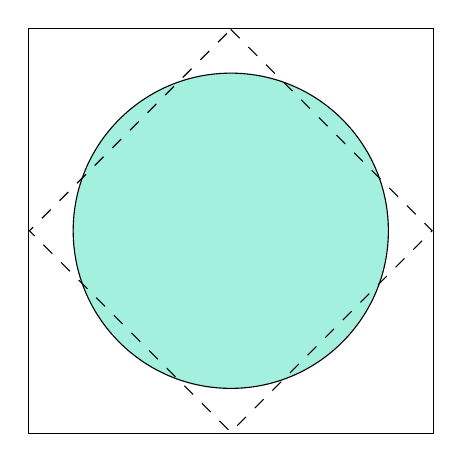
\begin{tikzpicture}[x=0.75pt,y=0.75pt,yscale=-1,xscale=1]
%uncomment if require: \path (0,300); %set diagram left start at 0, and has height of 300

%Shape: Square [id:dp2502427835904639] 
\draw   (241.83,21.67) -- (437,21.67) -- (437,216.83) -- (241.83,216.83) -- cycle ;
%Shape: Circle [id:dp1839510682473804] 
\draw  [fill={rgb, 255:red, 80; green, 227; blue, 194 }  ,fill opacity=0.52 ] (263.48,119.25) .. controls (263.48,77.31) and (297.48,43.31) .. (339.42,43.31) .. controls (381.36,43.31) and (415.35,77.31) .. (415.35,119.25) .. controls (415.35,161.19) and (381.36,195.19) .. (339.42,195.19) .. controls (297.48,195.19) and (263.48,161.19) .. (263.48,119.25) -- cycle ;
%Shape: Square [id:dp70425401409973] 
\draw  [dash pattern={on 4.5pt off 4.5pt}] (339.42,22.25) -- (436.42,119.25) -- (339.42,216.25) -- (242.42,119.25) -- cycle ;




\end{tikzpicture}

    }
    \subfigure[将格点划分为A格点和B格点之后的第一布里渊区和费米面,注意费米面和折叠了的第一布里渊区相交]{
        

\tikzset{every picture/.style={line width=0.75pt}} %set default line width to 0.75pt        

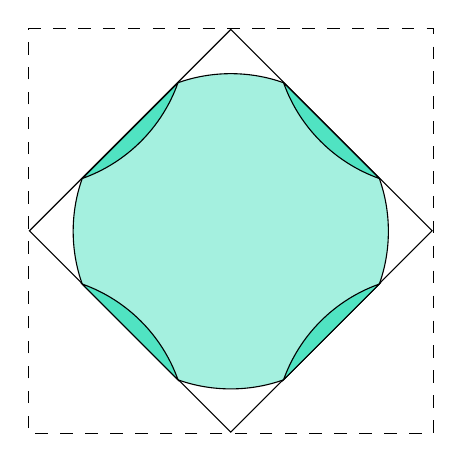
\begin{tikzpicture}[x=0.75pt,y=0.75pt,yscale=-1,xscale=1]
%uncomment if require: \path (0,259); %set diagram left start at 0, and has height of 259

%Shape: Square [id:dp11895947219652458] 
\draw  [dash pattern={on 4.5pt off 4.5pt}] (225.83,27.67) -- (421,27.67) -- (421,222.83) -- (225.83,222.83) -- cycle ;
%Shape: Square [id:dp8743886021547951] 
\draw   (323.42,28.25) -- (420.42,125.25) -- (323.42,222.25) -- (226.42,125.25) -- cycle ;
%Shape: Path Data [id:dp43269980232953076] 
\draw  [fill={rgb, 255:red, 80; green, 227; blue, 194 }  ,fill opacity=0.52 ] (323.42,49.56) .. controls (332.33,49.56) and (340.89,51.1) .. (348.84,53.92) -- (394.99,100.08) .. controls (397.82,108.03) and (399.35,116.58) .. (399.35,125.5) .. controls (399.35,134.42) and (397.82,142.97) .. (394.99,150.92) -- (348.84,197.08) .. controls (340.89,199.9) and (332.33,201.44) .. (323.42,201.44) .. controls (314.5,201.44) and (305.94,199.9) .. (297.99,197.08) -- (251.84,150.92) .. controls (249.02,142.97) and (247.48,134.42) .. (247.48,125.5) .. controls (247.48,116.58) and (249.02,108.03) .. (251.84,100.08) -- (297.99,53.92) .. controls (305.94,51.1) and (314.5,49.56) .. (323.42,49.56) -- cycle ;
%Shape: Path Data [id:dp9231670075411238] 
\draw  [fill={rgb, 255:red, 80; green, 227; blue, 194 }  ,fill opacity=1 ] (394.99,150.92) .. controls (373.51,158.55) and (356.47,175.59) .. (348.84,197.08) -- (394.99,150.92) -- cycle ;
%Shape: Path Data [id:dp01617091905340562] 
\draw  [fill={rgb, 255:red, 80; green, 227; blue, 194 }  ,fill opacity=1 ] (251.84,150.92) .. controls (273.33,158.55) and (290.36,175.59) .. (297.99,197.08) -- (251.84,150.92) -- cycle ;
%Shape: Path Data [id:dp9718706516418314] 
\draw  [fill={rgb, 255:red, 80; green, 227; blue, 194 }  ,fill opacity=1 ] (394.99,100.08) .. controls (373.51,92.45) and (356.47,75.41) .. (348.84,53.92) -- (394.99,100.08) -- cycle ;
%Shape: Path Data [id:dp9257995198566793] 
\draw  [fill={rgb, 255:red, 80; green, 227; blue, 194 }  ,fill opacity=1 ] (251.84,100.08) .. controls (273.33,92.45) and (290.36,75.41) .. (297.99,53.92) -- (251.84,100.08) -- cycle ;




\end{tikzpicture}

    }
    \subfigure[电子受到SDW序散射,导致能隙打开,出现两条能带,深绿的区域为费米口袋,这些区域同时有两个能带的电子填充]{
        

\tikzset{every picture/.style={line width=0.75pt}} %set default line width to 0.75pt        

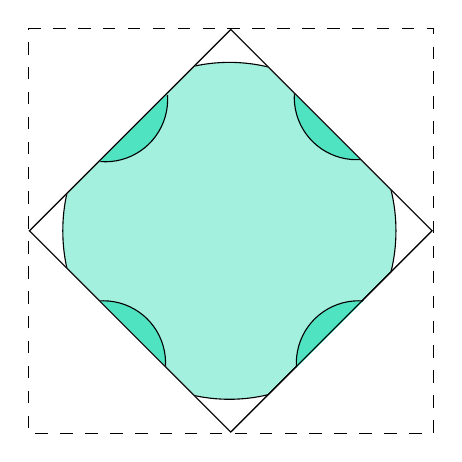
\begin{tikzpicture}[x=0.75pt,y=0.75pt,yscale=-1,xscale=1]
%uncomment if require: \path (0,300); %set diagram left start at 0, and has height of 300

%Shape: Path Data [id:dp6347441590753127] 
\draw  [fill={rgb, 255:red, 80; green, 227; blue, 194 }  ,fill opacity=0.52 ] (342.74,64.12) .. controls (349.21,64.12) and (355.5,64.9) .. (361.52,66.36) -- (420.58,125.41) .. controls (422.16,131.77) and (423,138.42) .. (423,145.28) .. controls (423,152.11) and (422.17,158.74) .. (420.6,165.07) -- (361.44,224.22) .. controls (355.44,225.67) and (349.18,226.44) .. (342.74,226.44) .. controls (336.93,226.44) and (331.25,225.81) .. (325.79,224.62) -- (264.46,163.3) .. controls (263.17,157.5) and (262.48,151.47) .. (262.48,145.28) .. controls (262.48,139.06) and (263.17,133) .. (264.48,127.19) -- (325.72,65.95) .. controls (331.2,64.75) and (336.9,64.12) .. (342.74,64.12) -- cycle ;
%Shape: Arc [id:dp9397326133788] 
\draw  [draw opacity=0][fill={rgb, 255:red, 80; green, 227; blue, 194 }  ,fill opacity=1 ] (406.41,110.91) .. controls (392.45,112.05) and (379.16,103.24) .. (375.16,89.25) .. controls (374.17,85.79) and (373.83,82.29) .. (374.07,78.89) -- (404,81) -- cycle ; \draw   (406.41,110.91) .. controls (392.45,112.05) and (379.16,103.24) .. (375.16,89.25) .. controls (374.17,85.79) and (373.83,82.29) .. (374.07,78.89) ;
%Shape: Square [id:dp49917369182880145] 
\draw   (343.42,48.25) -- (440.42,145.25) -- (343.42,242.25) -- (246.42,145.25) -- cycle ;
%Shape: Arc [id:dp8484610197939879] 
\draw  [draw opacity=0][fill={rgb, 255:red, 80; green, 227; blue, 194 }  ,fill opacity=1 ] (280.59,111.91) .. controls (294.55,113.05) and (307.84,104.24) .. (311.84,90.25) .. controls (312.83,86.79) and (313.17,83.29) .. (312.93,79.89) -- (283,82) -- cycle ; \draw   (280.59,111.91) .. controls (294.55,113.05) and (307.84,104.24) .. (311.84,90.25) .. controls (312.83,86.79) and (313.17,83.29) .. (312.93,79.89) ;
%Shape: Arc [id:dp6476837513798173] 
\draw  [draw opacity=0][fill={rgb, 255:red, 80; green, 227; blue, 194 }  ,fill opacity=1 ] (407.41,179.09) .. controls (393.45,177.95) and (380.16,186.76) .. (376.16,200.75) .. controls (375.17,204.21) and (374.83,207.71) .. (375.07,211.11) -- (405,209) -- cycle ; \draw   (407.41,179.09) .. controls (393.45,177.95) and (380.16,186.76) .. (376.16,200.75) .. controls (375.17,204.21) and (374.83,207.71) .. (375.07,211.11) ;
%Shape: Arc [id:dp5512282331487339] 
\draw  [draw opacity=0][fill={rgb, 255:red, 80; green, 227; blue, 194 }  ,fill opacity=1 ] (279.59,179.09) .. controls (293.55,177.95) and (306.84,186.76) .. (310.84,200.75) .. controls (311.83,204.21) and (312.17,207.71) .. (311.93,211.11) -- (282,209) -- cycle ; \draw   (279.59,179.09) .. controls (293.55,177.95) and (306.84,186.76) .. (310.84,200.75) .. controls (311.83,204.21) and (312.17,207.71) .. (311.93,211.11) ;
%Shape: Right Triangle [id:dp2444716275585217] 
\draw  [color={rgb, 255:red, 255; green, 255; blue, 255 }  ,draw opacity=1 ][fill={rgb, 255:red, 255; green, 255; blue, 255 }  ,fill opacity=1 ] (246.42,145.25) -- (343.42,48.25) -- (246.42,48.25) -- cycle ;
%Shape: Right Triangle [id:dp7467362132163622] 
\draw  [color={rgb, 255:red, 255; green, 255; blue, 255 }  ,draw opacity=1 ][fill={rgb, 255:red, 255; green, 255; blue, 255 }  ,fill opacity=1 ] (440.42,145.25) -- (343.42,48.25) -- (440.42,48.25) -- cycle ;
%Shape: Right Triangle [id:dp8978210412148069] 
\draw  [color={rgb, 255:red, 255; green, 255; blue, 255 }  ,draw opacity=1 ][fill={rgb, 255:red, 255; green, 255; blue, 255 }  ,fill opacity=1 ] (441,145.83) -- (344,242.83) -- (441,242.83) -- cycle ;
%Shape: Right Triangle [id:dp5172920566536954] 
\draw  [color={rgb, 255:red, 255; green, 255; blue, 255 }  ,draw opacity=1 ][fill={rgb, 255:red, 255; green, 255; blue, 255 }  ,fill opacity=1 ] (247,145.83) -- (344,242.83) -- (247,242.83) -- cycle ;
%Shape: Square [id:dp19483120370981322] 
\draw   (343.42,48.25) -- (440.42,145.25) -- (343.42,242.25) -- (246.42,145.25) -- cycle ;
%Shape: Square [id:dp47724188658303346] 
\draw  [dash pattern={on 4.5pt off 4.5pt}] (245.83,47.67) -- (441,47.67) -- (441,242.83) -- (245.83,242.83) -- cycle ;




\end{tikzpicture}
    }
    \subfigure[热点]{
        

\tikzset{every picture/.style={line width=0.75pt}} %set default line width to 0.75pt        

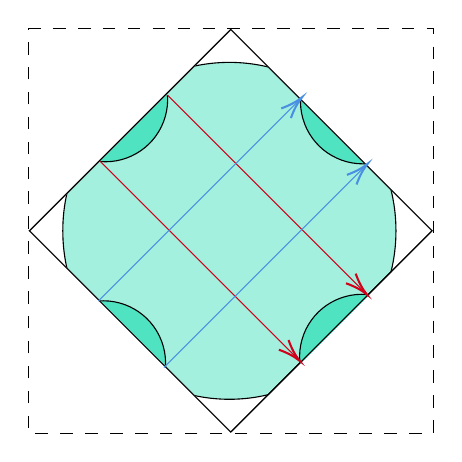
\begin{tikzpicture}[x=0.75pt,y=0.75pt,yscale=-1,xscale=1]
%uncomment if require: \path (0,300); %set diagram left start at 0, and has height of 300

%Shape: Path Data [id:dp28391475851762316] 
\draw  [fill={rgb, 255:red, 80; green, 227; blue, 194 }  ,fill opacity=0.52 ] (325.74,53.12) .. controls (332.21,53.12) and (338.5,53.9) .. (344.52,55.36) -- (403.58,114.41) .. controls (405.16,120.77) and (406,127.42) .. (406,134.28) .. controls (406,141.11) and (405.17,147.74) .. (403.6,154.07) -- (344.44,213.22) .. controls (338.44,214.67) and (332.18,215.44) .. (325.74,215.44) .. controls (319.93,215.44) and (314.25,214.81) .. (308.79,213.62) -- (247.46,152.3) .. controls (246.17,146.5) and (245.48,140.47) .. (245.48,134.28) .. controls (245.48,128.06) and (246.17,122) .. (247.48,116.19) -- (308.72,54.95) .. controls (314.2,53.75) and (319.9,53.12) .. (325.74,53.12) -- cycle ;
%Shape: Arc [id:dp4924996181571455] 
\draw  [draw opacity=0][fill={rgb, 255:red, 80; green, 227; blue, 194 }  ,fill opacity=1 ] (392.41,101.91) .. controls (378.45,103.05) and (365.16,94.24) .. (361.16,80.25) .. controls (360.17,76.79) and (359.83,73.29) .. (360.07,69.89) -- (390,72) -- cycle ; \draw   (392.41,101.91) .. controls (378.45,103.05) and (365.16,94.24) .. (361.16,80.25) .. controls (360.17,76.79) and (359.83,73.29) .. (360.07,69.89) ;
%Shape: Square [id:dp8258883831288684] 
\draw   (326.42,37.25) -- (423.42,134.25) -- (326.42,231.25) -- (229.42,134.25) -- cycle ;
%Shape: Arc [id:dp34996890506368183] 
\draw  [draw opacity=0][fill={rgb, 255:red, 80; green, 227; blue, 194 }  ,fill opacity=1 ] (263.59,100.91) .. controls (277.55,102.05) and (290.84,93.24) .. (294.84,79.25) .. controls (295.83,75.79) and (296.17,72.29) .. (295.93,68.89) -- (266,71) -- cycle ; \draw   (263.59,100.91) .. controls (277.55,102.05) and (290.84,93.24) .. (294.84,79.25) .. controls (295.83,75.79) and (296.17,72.29) .. (295.93,68.89) ;
%Shape: Arc [id:dp4561026088076878] 
\draw  [draw opacity=0][fill={rgb, 255:red, 80; green, 227; blue, 194 }  ,fill opacity=1 ] (392,164.96) .. controls (378.04,163.82) and (364.75,172.63) .. (360.75,186.61) .. controls (359.75,190.08) and (359.41,193.58) .. (359.65,196.97) -- (389.59,194.87) -- cycle ; \draw   (392,164.96) .. controls (378.04,163.82) and (364.75,172.63) .. (360.75,186.61) .. controls (359.75,190.08) and (359.41,193.58) .. (359.65,196.97) ;
%Shape: Arc [id:dp15892708580174042] 
\draw  [draw opacity=0][fill={rgb, 255:red, 80; green, 227; blue, 194 }  ,fill opacity=1 ] (262.59,168.09) .. controls (276.55,166.95) and (289.84,175.76) .. (293.84,189.75) .. controls (294.83,193.21) and (295.17,196.71) .. (294.93,200.11) -- (265,198) -- cycle ; \draw   (262.59,168.09) .. controls (276.55,166.95) and (289.84,175.76) .. (293.84,189.75) .. controls (294.83,193.21) and (295.17,196.71) .. (294.93,200.11) ;
%Shape: Right Triangle [id:dp9873621257073468] 
\draw  [color={rgb, 255:red, 255; green, 255; blue, 255 }  ,draw opacity=1 ][fill={rgb, 255:red, 255; green, 255; blue, 255 }  ,fill opacity=1 ] (229.42,134.25) -- (326.42,37.25) -- (229.42,37.25) -- cycle ;
%Shape: Right Triangle [id:dp20784307542005132] 
\draw  [color={rgb, 255:red, 255; green, 255; blue, 255 }  ,draw opacity=1 ][fill={rgb, 255:red, 255; green, 255; blue, 255 }  ,fill opacity=1 ] (423.42,134.25) -- (326.42,37.25) -- (423.42,37.25) -- cycle ;
%Shape: Right Triangle [id:dp19958209753051315] 
\draw  [color={rgb, 255:red, 255; green, 255; blue, 255 }  ,draw opacity=1 ][fill={rgb, 255:red, 255; green, 255; blue, 255 }  ,fill opacity=1 ] (424,134.83) -- (327,231.83) -- (424,231.83) -- cycle ;
%Shape: Right Triangle [id:dp13150240831757665] 
\draw  [color={rgb, 255:red, 255; green, 255; blue, 255 }  ,draw opacity=1 ][fill={rgb, 255:red, 255; green, 255; blue, 255 }  ,fill opacity=1 ] (230,134.83) -- (327,231.83) -- (230,231.83) -- cycle ;
%Shape: Square [id:dp6591394813744926] 
\draw   (326.42,37.25) -- (423.42,134.25) -- (326.42,231.25) -- (229.42,134.25) -- cycle ;
%Shape: Square [id:dp30244562238327477] 
\draw  [dash pattern={on 4.5pt off 4.5pt}] (228.83,36.67) -- (424,36.67) -- (424,231.83) -- (228.83,231.83) -- cycle ;
%Straight Lines [id:da43761852194250594] 
\draw [color={rgb, 255:red, 208; green, 2; blue, 27 }  ,draw opacity=1 ]   (295.93,68.89) -- (390.59,163.54) ;
\draw [shift={(392,164.96)}, rotate = 225] [color={rgb, 255:red, 208; green, 2; blue, 27 }  ,draw opacity=1 ][line width=0.75]    (10.93,-3.29) .. controls (6.95,-1.4) and (3.31,-0.3) .. (0,0) .. controls (3.31,0.3) and (6.95,1.4) .. (10.93,3.29)   ;
%Straight Lines [id:da018143618520460425] 
\draw [color={rgb, 255:red, 208; green, 2; blue, 27 }  ,draw opacity=1 ]   (263.59,100.91) -- (358.24,195.56) ;
\draw [shift={(359.65,196.97)}, rotate = 225] [color={rgb, 255:red, 208; green, 2; blue, 27 }  ,draw opacity=1 ][line width=0.75]    (10.93,-3.29) .. controls (6.95,-1.4) and (3.31,-0.3) .. (0,0) .. controls (3.31,0.3) and (6.95,1.4) .. (10.93,3.29)   ;
%Straight Lines [id:da48286677460832284] 
\draw [color={rgb, 255:red, 74; green, 144; blue, 226 }  ,draw opacity=1 ]   (262.59,168.09) -- (359.37,71.31) ;
\draw [shift={(360.79,69.89)}, rotate = 495] [color={rgb, 255:red, 74; green, 144; blue, 226 }  ,draw opacity=1 ][line width=0.75]    (10.93,-3.29) .. controls (6.95,-1.4) and (3.31,-0.3) .. (0,0) .. controls (3.31,0.3) and (6.95,1.4) .. (10.93,3.29)   ;
%Straight Lines [id:da3902094286940192] 
\draw [color={rgb, 255:red, 74; green, 144; blue, 226 }  ,draw opacity=1 ]   (294.21,200.11) -- (391,103.32) ;
\draw [shift={(392.41,101.91)}, rotate = 495] [color={rgb, 255:red, 74; green, 144; blue, 226 }  ,draw opacity=1 ][line width=0.75]    (10.93,-3.29) .. controls (6.95,-1.4) and (3.31,-0.3) .. (0,0) .. controls (3.31,0.3) and (6.95,1.4) .. (10.93,3.29)   ;




\end{tikzpicture}
    }
    \caption{布里渊区折叠和费米口袋形成}
\end{figure}

如果费米面和折叠后的第一布里渊区相交,费米面交叉处打开能隙,形成一系列小的费米口袋。热点附近的$\vb*{k}$和$\vb*{k} + \vb*{Q}$都在热点附近。

接下来讨论在热点附近的低能有效理论,换而言之,我们开始讨论超越平均场的物理。
需要注意的是考虑超越平均场的物理意味着将原本被忽略的涨落重新加入,这可能改变热点的位置或者甚至让热点消失(在本问题中不可能因为涨落不大,但确实有这样的体系,涨落会让平均场理论中出现的现象——如相变——消失,比如一维伊辛模型)。
因此,下面讨论的热点附近的低能有效理论建立在三个基础上:
\begin{enumerate}
    \item 费米面上存在热点,这是通过平均场理论算出来的,我们假定这个现象确实存在,而不是像一维伊辛模型一样只是幻象;
    \item 热点附近的低能有效理论是\eqref{eq:2dim-square-spin}的低能有效理论,即相互作用项一定是自旋-自旋相互作用(这并非假设,而是必然的事实);
    \item 低能自由度是低能电子和自旋波模式这两种场(实际上这是最重要的一个假设,因为低能自由度是什么通常难以直接计算得到)。
\end{enumerate}

\eqref{eq:2dim-square-spin}中的相互作用项是一个电子和一个自旋波模式(这是玻色子)发生散射,得到另一个电子,或者也可以说是自由电子的自旋和自旋波模式的相互作用。%
\footnote{自旋波模式是一部分形成了自旋波的电子被积掉之后得到的,和未形成自旋波长程序的电子是两群不同的电子。}%
因此低能有效理论的散射项形如%
\footnote{一个可能的问题是,为什么一定保留低能电子自由度和自旋波自由度?为什么不能是自旋波自由度和密度波自由度?不考虑自旋波-密度波自由度是因为没有明确的物理机制让这两个模式发生耦合,保留低能电子自由度是因为自旋算符和电子数算符对易,但和单个费米子算符并不对易,因此可能出现费米子自由度积不掉的情况。
这和BCS理论是不一样的,在BCS理论中大量电子参与配对,以至于哪怕电子自由度积不掉,它也不会产生太大作用。}%
\[
    {\phi}_{\vb*{q}} {c}^\dagger_{\vb*{k}+\vb*{q}\sigma} {c}_{\vb*{k}\sigma'},
\]
由于是低能有效理论,我们认为形成了一个基本上稳定的反铁磁序,于是$\vb*{q}$接近$\vb*{Q}$,而电子能量$\epsilon_{\vb*{k}}$和$\epsilon_{\vb*{k}+\vb*{q}}$都在费米面附近。
这些条件只有在热点附近才能达到。
当然由于热点是费米面交叠之后打开能隙的位置,在这附近有低能有效理论是非常合理的。
这样,一个散射过程涉及两个热点。分别用1和2标记两个热点,记它们的动量为$\vb*{K}_1$和$\vb*{K}_2$,则有
\[
    \vb*{K}_2 = \vb*{K}_1 + \vb*{Q},
\]
并重新定义$\vb*{q}$和$\vb*{k}$为它们偏离$\vb*{Q}$和$\vb*{K}_1$的大小。这样,相互作用哈密顿量就是
\[
    {\vb*{\phi}}_{\vb*{q}} \cdot (\sum_{\alpha, \beta} {c}^\dagger_{1(\vb*{k} + \vb*{q})\alpha} \vb*{\sigma}_{\alpha \beta} {c}_{2\vb*{k} \beta} + \text{h.c.}),
\]
这里任何一个散射过程中入射电子为热点1附加,出射电子在热点2附加或相反的原因是要保证所有电子的动量都在热点附加。于是完整的有效理论的哈密顿量为
\begin{equation}
    {H}_\text{eff} = \sum_{\vb*{k}, \sigma} (\xi_{1\vb*{k}} {c}^\dagger_{1\vb*{k} \sigma} {c}_{1 \vb*{k} \sigma} + \xi_{2\vb*{k}} {c}^\dagger_{2\vb*{k} \sigma} {c}_{2 \vb*{k} \sigma}) + {H}[\vb*{\phi}] + \lambda \sum_{\vb*{q}} {\vb*{\phi}}_{\vb*{q}} \cdot (\sum_{\alpha, \beta} {c}^\dagger_{1(\vb*{k} + \vb*{q})\alpha} \vb*{\sigma}_{\alpha \beta} {c}_{2\vb*{k} \beta} + \text{h.c.}).
    \label{eq:2dim-square-spin-eff}
\end{equation}
上式中没有明确提玻色场——也就是自旋波场——的自由哈密顿量。这个自由哈密顿量通常是通过对称性分析得出的。
进一步,由于是低能理论,将$\xi_{\vb*{k}}$在费米面附近做展开,仅保留一阶项,得到
\begin{equation}
    \xi_{1\vb*{k}} = \epsilon_{\vb*{k}} - \mu = \vb*{v}_1 \cdot \vb*{k}, \quad \xi_{2\vb*{k}} = \epsilon_{\vb*{k}} - \mu = \vb*{v}_2 \cdot \vb*{k}.
\end{equation}
使用$\vb*{v}_1$和$\vb*{v}_2$来标记$\grad_{\vb*{k}}{\xi_{\vb*{k}}}$是因为如果是自由电子气,那么它们就是费米速度。

\subsection{朗道阻尼}

现在我们尝试把电子完全积掉,只留下玻色型的自旋波模式。需要指出的是这个操作并不总是可行的:由于自旋波模式和电子都是低能自由度,简单地积掉其中一个自由度可能不能得到一个良定义的有效理论。
实际上,对二维体系的确会有这种棘手的细节。
下面的操作都是在默认确实可以积掉电子的前提下进行的。

从\eqref{eq:2dim-square-spin-eff}可以看出,一个自旋波模式可以衰变成一对电子空穴对,或者说一个自旋波模式可以将动量转移给一个电子而得到另一个电子,而自身湮灭。
因此自旋波模式是有有限的寿命的。由费米黄金法则,一个动量为$\vb*{q}$,能量为大于零的$\omega$的自旋波模式的寿命倒数为
\[
    \begin{aligned}
        \frac{1}{\tau} &\sim 2 \lambda^2 \int \frac{\dd[2]{\vb*{k}}}{(2\pi)^2} \delta(\omega + \epsilon_{1 \vb*{k}} - \epsilon_{2 (\vb*{k} + \vb*{q})}) \theta(- \epsilon_{1 \vb*{k}}) \theta(\epsilon_{2 (\vb*{k} + \vb*{q})}) \\
        &\sim \lambda^2 \int \frac{\dd{p_1} \dd{p_2}}{(2\pi)^2 \abs*{\vb*{v}_1 \times \vb*{v}_2}} \delta(\omega + p_1 - p_2) \theta(- p_1) \theta(p_2),
    \end{aligned}
\]
其中我们设
\[
    p_1 = \vb*{v}_1 \cdot \vb*{k}, \quad p_2 = \vb*{v}_2 \cdot (\vb*{k} + \vb*{q}),
\]
我们仅考虑低能理论,因此假定入射电子在费米面以下,出射电子在费米面以上。由几何关系,
\[
    \int \frac{\dd{p_1} \dd{p_2}}{\abs*{\vb*{v}_1 \times \vb*{v}_2}} \delta(\omega + p_1 - p_2) \theta(- p_1) \theta(p_2) = \sqrt{2} \omega,
\]
$\omega < 0$的情况也是一样的。总之最后自旋波模式的寿命为
\begin{equation}
    \frac{1}{\tau} \sim \frac{\lambda^2}{\abs*{\vb*{v}_1 \times \vb*{v}_2}} \abs*{\omega} = \gamma \abs*{\omega}.
\end{equation}
在格林函数中,衰变几率对应着自能修正,会直接反映在$\vb*{\phi}$的格林函数——从而有效作用量——中,也即,自旋波模式的推迟格林函数形如
\[
    G_{\vb*{\phi}}^{-1} = \ii \gamma \abs{\omega} + \cdots = \ii  \gamma \sgn(\omega) \omega + \cdots,
\]
相应的,松原格林函数形式为%
\footnote{这里的步骤是:先做Wick转动,即$\omega = \ii \omega_n$,}%
\[
    G_{\vb*{\phi}}^{-1} = \gamma \abs{\omega_n} + \cdots.
\]
这就意味着自旋波模式的有效热力学作用量为
\begin{equation}
    \begin{aligned}
        S_\text{eff} &= \sum_{\vb*{q}, \omega_n} \vb*{\phi}(-\vb*{q}, -\omega_n) \cdot (\gamma \abs{\omega_n} + \omega_n^2 + c^2 \vb*{q}^2 ) \vb*{\phi}(\vb*{q}, \omega_n) \\
        &= \sum_{\vb*{q}, \omega_n} \vb*{\phi}^*(\vb*{q}, \omega_n) \cdot (\gamma \abs{\omega_n} + \omega_n^2 + c^2 \vb*{q}^2) \vb*{\phi}(\vb*{q}, \omega_n).
    \end{aligned}
    \label{eq:effective-spin-action}
\end{equation}
第二个等号是因为$\vb*{\phi}$是实场,因为负的动量/频率等价于取复共轭。
$\omega_n^2$项和$\vb*{q}^2$项都是对称性分析加入的项,除此以外的项在低能有效理论中并不重要。%
$\omega_n^2$项和$\vb*{k}^2$项可以容易地切换到实空间,它们分别对应着时间导数平方项$(\partial_\tau \phi)^2$和梯度平方项$(\grad{\phi})^2$,但$\abs{\omega_n}$在实空间中没有简单的形式。
不过,一个正比于$\omega_n$的项意味着实空间中有某种阻尼,这也是正确的,因为自旋波模式如前所述会衰变。这种阻尼或者衰变称为\concept{朗道阻尼}。朗道阻尼指的是没有粒子之间的相互碰撞,仅仅粒子和波强烈耦合也能够产生阻尼。

\subsection{RPA近似计算朗道阻尼}

还可以通过直接计算格林函数的方式来得到$\phi$的有效理论。
这个有效理论当然取
\[
    Z_\text{eff} = \int \mathcal{D}\vb*{\phi} \ee^{- \sum_{q, \omega_n} \vb*{\phi}^*(\vb*{q}, \omega_n) G^{-1}_{\vb*{\phi}}(\vb*{q}, \omega_n) \vb*{\phi}(\vb*{q}, \omega_n)}
\]
的形式。

\subsection{Hertz理论}

最后我们讨论上一节得到的低能有效理论的

\subsection{RPA近似}

我们尝试对平均场近似做一些修正。为此我们将不再直接处理自旋算符,而是把一切都转化到费米子算符上。
做傅里叶变换
\[
    {S}_{\vb*{q}} = \frac{1}{\sqrt{N_\text{site}}} \sum_{\vb*{i}} {S}_i \ee^{\ii \vb*{r}_i \cdot \vb*{q}} = \frac{1}{\sqrt{N_\text{site}}} \sum_{\vb*{k}} {c}^\dagger_{\vb*{k}+\vb*{q}, \alpha} \vb*{\sigma}_{\alpha \beta} {c}_{\vb*{k} \beta},
\]
这样相互作用项就是(请注意$\vb*{\sigma}$)

对相互作用项做正规序不会影响定性的结果,我们不需要动手算就知道正规序和原本的相互作用只会差一个单体项,而这个单体项是自选旋转不变的,那么它只会对$\epsilon_{\vb*{k}} - \mu$做一个修正。
于是我们将要处理以下相互作用哈密顿量:% TODO:自旋
\begin{equation}
    {H} = \frac{1}{2 N_\text{site}} \sum_{\vb*{k}, \vb*{k}', \vb*{q}, \alpha, \beta} {c}^\dagger_{\vb*{k}-\vb*{q}, \alpha} {c}^\dagger_{\vb*{k}'+\vb*{q}, \beta} V(\vb*{q}) {c}_{\vb*{k}'} {c}_{\vb*{k}}, \quad V(\vb*{q}) = 2 J (\cos(q_x) + \cos(q_y)).
\end{equation}

\begin{equation}
    Z = \int \fd{\vb*{\phi}} \exp(- \int_0^\beta \dd{\tau} )
\end{equation}

$\vb*{\phi}$就像驱动自旋的一个外场一样,在只取鞍点近似时它就是平均场序参量。